% !TeX root = dissertation.tex
\chapter{ISA virtualization is untenable for GPUs}
\label{sec:trillium}

\begin{figure}[!th]
	\centering
	% \begin{subfigure}{0.25\linewidth}
	% 	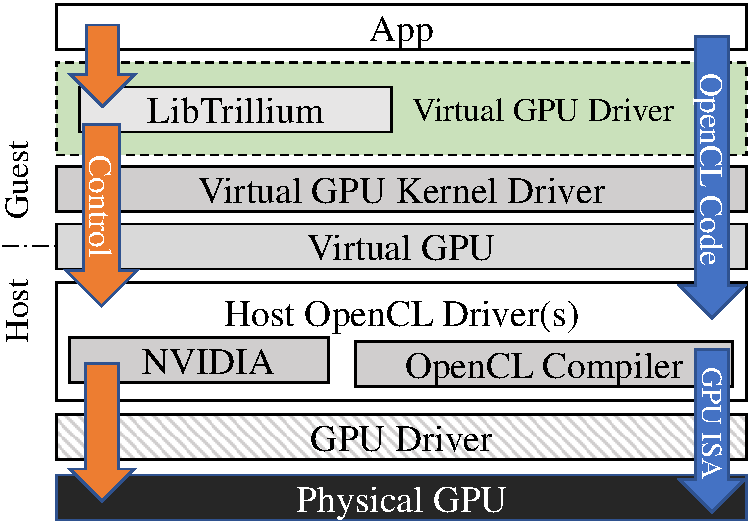
\includegraphics[width=\linewidth,trim={0cm 0cm 0cm 0cm},clip]{figures/trillium_design.pdf}
	% 	\caption{{}}
	% 	\label{fig_trillium}
	% \end{subfigure}\hfill
	\begin{subfigure}{0.45\linewidth}
		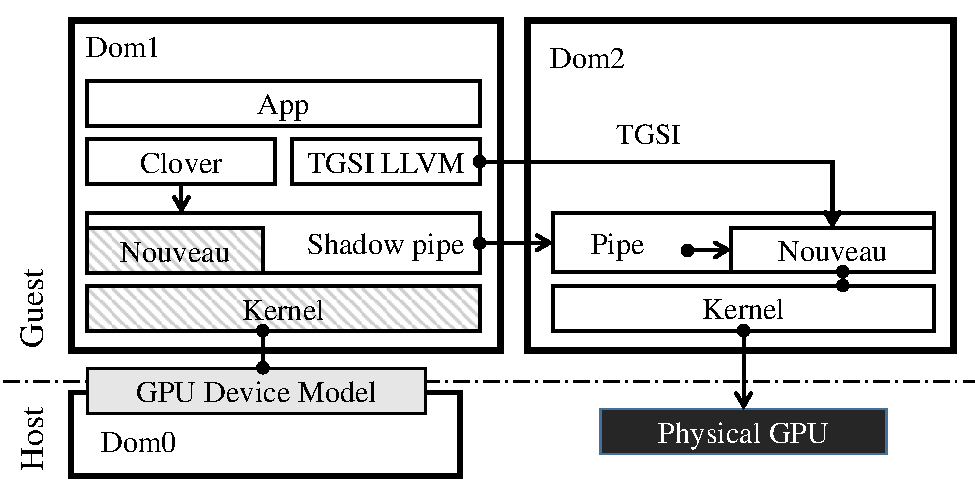
\includegraphics[width=\linewidth,trim={0 0 0 0},clip]{figures/xen-svga.pdf}
		\caption{{}}
		\label{fig_xen_svga}
	\end{subfigure}\hfill
	\begin{subfigure}{0.45\linewidth}
		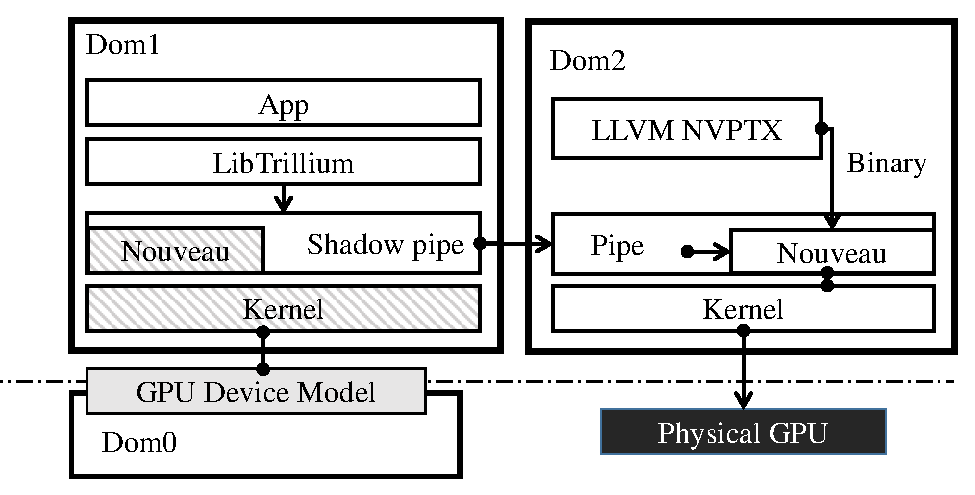
\includegraphics[width=\linewidth,trim={0.6cm 0 0 0},clip]{figures/trillium.pdf}
		\caption{{}}
		\label{fig_trillium}
	\end{subfigure}
	\caption{Xen-SVGA and Trillium designs. (a) The Trillium stack. (b) Xen-SVGA approximates the SVGA model extended to support GPU Compute. (c) The design of Trillium with shadow pipe.}
\end{figure}

In many parallel computing domains, compute density and
programmability~\cite{nvidia_cuda, stone2010opencl, gregory2014c++} have
made GPUs the clear choice for efficiency and performance~\cite{gpu_apps}.
Popular machine learning frameworks such as Caffe~\cite{jia2014caffe},
Tensorflow~\cite{abadi2016tensorflow}, CNTK~\cite{yu2014introduction}, and
Torch7~\cite{collobert2011torch7} rely on GPU acceleration heavily. GPUs have
made significant inroads in HPC as well: five of the top seven supercomputers
in the world are powered by GPUs~\cite{top500-Nov2018}.

Despite much prior research~\cite{rossbach16vee, kaveri16vee,
cc-numa-gpu-hpca15, abhishek-ispass16} on GPGPU virtualization, practical
options currently available to providers of virtual infrastructure all involve
bypassing the hypervisor.
The most commonly adopted technique is to dedicate GPUs to single VM instances
via PCIe pass-through~\cite{AWS-gpu,gVirt}, thereby giving up the
consolidation and fault tolerance benefits of virtualization.
More recently, industry players such as VMware, Dell and BitFusion have
introduced user-space API-remoting~\cite{bitfusion-whitepaper,kim2012snucl,
rCUDAnew, vmCUDA,rCUDA} based solutions as an alternative to pass-through.
API-remoting recovers the consolidation and encapsulation benefits
of virtualization but bypasses hypervisor interposition.
The absence of hypervisor interposition results in multiple disjoint resource
managers (the remote user-space API executor and the hypervisor) with no
insight into each others' decisions, thereby leading to poor decision making,
and priority-inversion problems~\cite{rossbach2011ptask}.

To recover hypervisor interposition while maintaining low-overhead,
we retrofit GPGPU support into a virtual GPU device:
We added support for OpenCL to an implementation of the
SVGA~\cite{dowty2009gpu} design in Xen (shown in Figure~\ref{fig_xen_svga}),
by implementing the key missing component---a compiler for SVGA's TGSI virtual
ISA.

\begin{figure}[!ht]
	\centering
	\captionsetup{width=0.8\linewidth}
	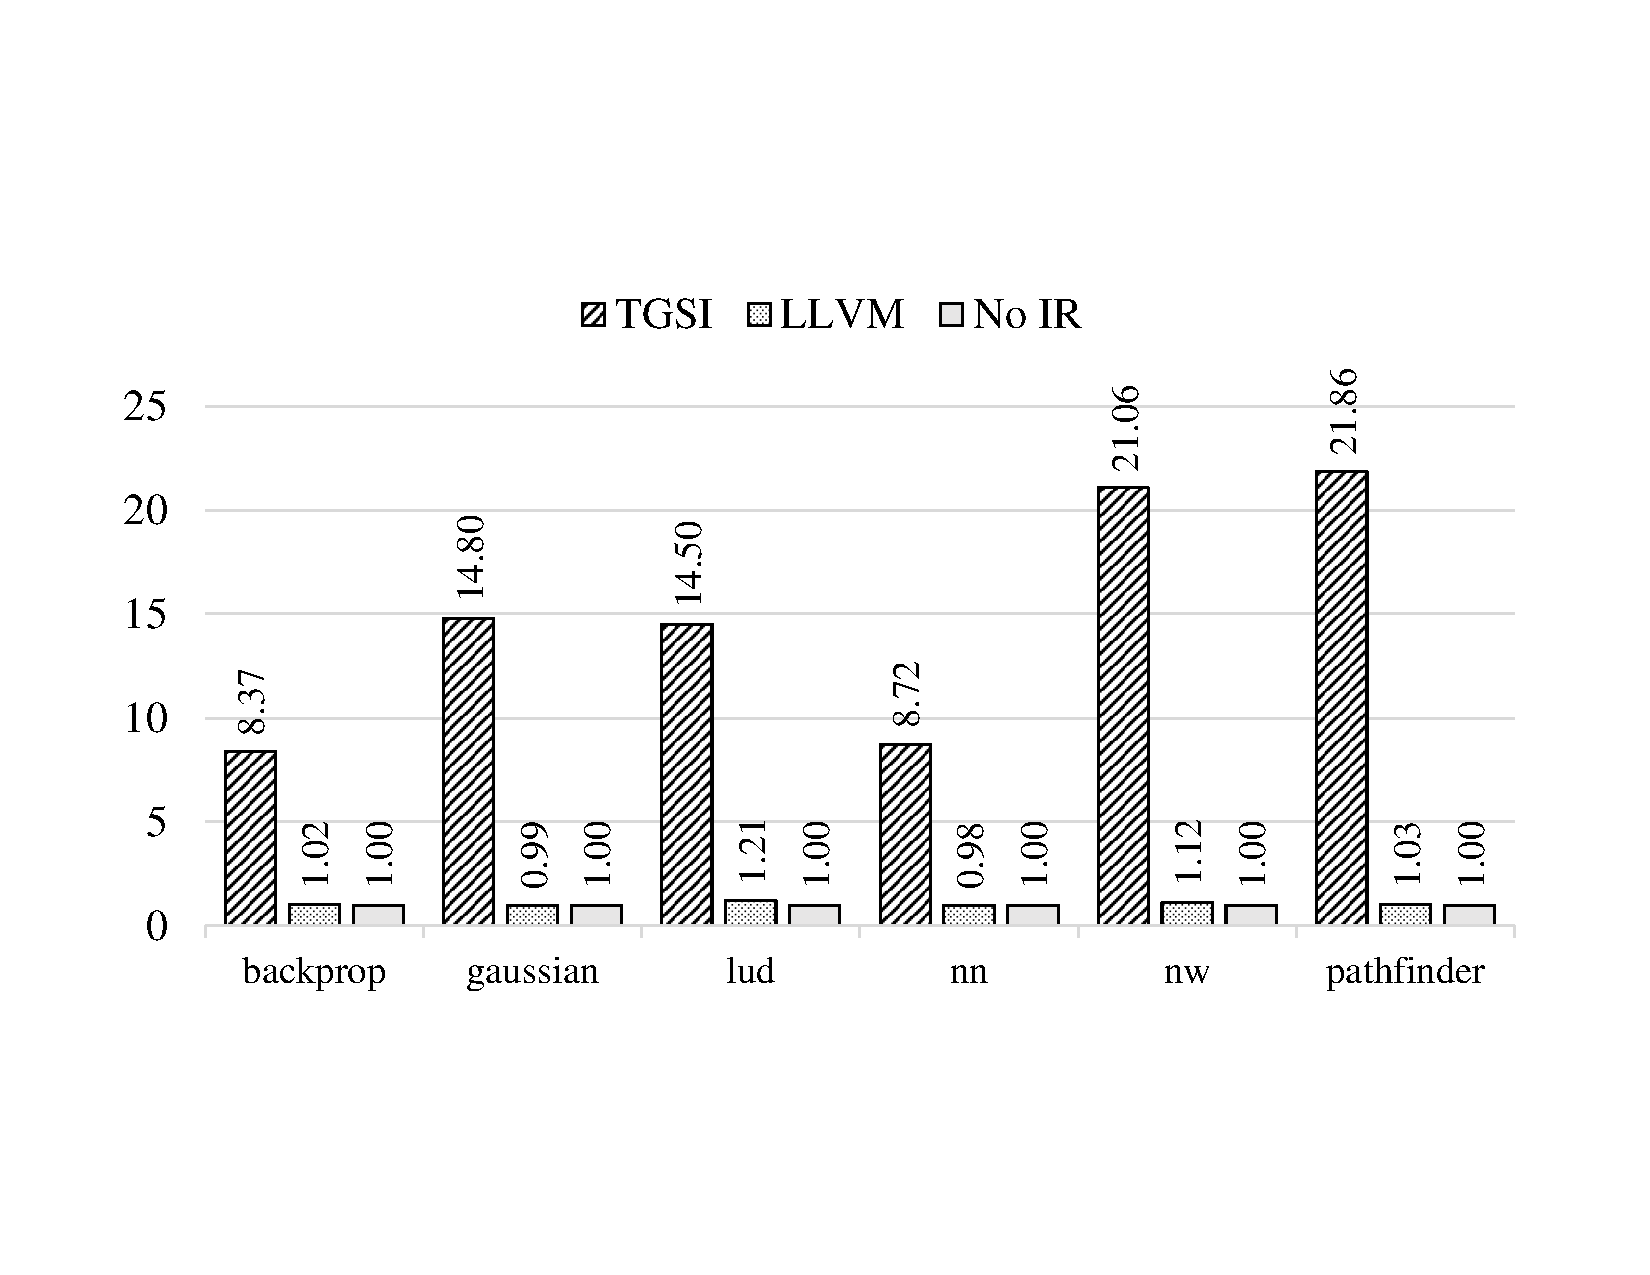
\includegraphics[width=.6\linewidth,trim={2cm 4.5cm 2cm 5cm},clip]{figures/trillium_visa.pdf}
	\caption{
		Kernel execution slowdown due to virtual ISAs.
		\textbf{TGSI}: the LLVM TGSI back-end compiler used in Xen-SVGA.
		\textbf{LLVM}: LLVM NVPTX back-end used in Trillium.
		\textbf{No IR}: native NVIDIA compiler.
		}
	\label{fig_trillium_kernel}
\end{figure}

This effort helped us realize that because GPUs already support vendor-specific
virtual ISAs (vISAs), the additional vISA provides little benefit.
Instead, we found that it harms performance, as shown in
Figure~\ref{fig_trillium_kernel}, by necessitating a translation layer that
obscures the program's semantic information from the final vendor-provided
compiler.
Drawing on this lesson, we adapted Trillium to take a more flexible approach
to ISA virtualization: eliding it entirely when the host GPU stack bundles a
compiler (most do), and using LLVM IR, when necessary, to provide a common
target for GPGPU drivers. Figure~\ref{fig_trillium} visually presents the
Trillium design.

Trillium is an existence proof of a viable alternative
design---hypervisor-mediated API-remoting---that preserves
desirable virtualization properties such as consolidation, hypervisor
interposition, isolation, encapsulation, etc., without requiring full hardware
virtualization.
While Trillium outperforms GPUvm~\cite{suzuki2014gpuvm}, a full virtualization
system, by up to 14$\times$ (5.5$\times$ on average) and the para-virtual
SVGA-like design by as much as 7.3$\times$ (5.4$\times$ on average), it
performs worse than a userspace API-remoting framework on average. We believe
this is because of a poor choice of API to forward: Trillium forwards the
nuoveau kernel graphics driver API, which is low enough in the stack that each
each userspace API function is broken into multiple RPC calls. A better
approach would be to forward the userspace API itself (presented in the next
chapter).

Concretely, this chapter will show that ISA virtualization is harmful for GPU
virtualization, and will lay the groundwork for a new hypothesis---%
Hypervisor-mediated API-remoting (of the user-space programming framework API)
is a realizable, performant, safe and composable virtualization scheme for
API-controlled accelerators.

The proposed chapter will draw material from joint work~\cite{trillium} with
Hangchen Yu, Arthur M. Peters, and Christopher J. Rossbach, and is likely to
appear in both my and Hangchen's dissertations. We have agreed to split the
work thus: My dissertation will focus on the inviability of ISA virtualization
while Hangchen will primarily use the findings of the paper (especially the
cross-product analysis of virtualization techniques) as motivation for
virtualization via API-remoting. His dissertation is focused on design and
implementation of API-remoting systems as enablers of access to accelerators
from both Virtual Machines and the OS kernel.